\documentclass{articleteyet}
%Para utilizar el proyecto como Template.
%- Loguearse,
%- Menú -> Copy Proyect
\usepackage[a4paper,left=2cm,right=2cm,top=3.5cm,bottom=2cm]{geometry}


\usepackage[latin1,utf8]{inputenc} 

%Comente la línea que continúa si su artículo está escrito en ingles.  Comment on the line that continues if your article is written in English  
\usepackage[spanish]{babel}

\usepackage{balance}
\usepackage{times}
\usepackage{hyperref}
\usepackage{graphicx}
 \usepackage{float}




\pagestyle{empty}


\title{Competencia de Programación en Bloques Colaborativa}

\author{
  Stacco Joan Manuel$^{1}$ \and Kogan Pablo$^{1}$ \and Godoy Ingrid$^{1}$ \and    Rodríguez Jorge$^{1}$ }
   


\infauthor{\emph{ $^{1}$ Facultad de Informática Universidad Nacional del Comahue}\\ \vspace{0.25cm} 
%\emph{ $^{2}$Filiación 2}\\
% \vspace{0.25cm} 
 {\tt joan.stacco@est.fi.uncoma.edu.ar, pablo.kogan@fi.uncoma.edu.ar, ingrid.godoy@fi.uncoma.edu.ar,  j.rodrig@fi.uncoma.edu.ar} 
} 


\begin{document}

\balance
\maketitle


\begin{abstract}
% 1/6 tiene esta sección


Desde que las Ciencias de la Computación se incluyeron como contenido en la escolaridad obligatoria, es importante trabajar sobre modelos didácticos, herramientas y estrategias que ayuden en la enseñanza y el aprendizaje de esta ciencia, para facilitar a los estudiantes la comprensión de estos conocimientos. En este documento presentaremos a la herramienta Hornero como gestor de torneos de programación en su nueva versión, que posibilita el desarrollo de programas en bloques, de forma colaborativa, con una interfaz responsive que permite a los docentes crear sus propios torneos, problemas y hacer seguimiento de las resoluciones provistas por los estudiantes.
Hornero es un sistema desarrollado  por estudiantes, docentes y graduados de la Universidad Nacional del Comahue que implementa un modelo de enseñanza y aprendizaje lúdico y colectivo, a través de competencias de programación.  
  

%para abajo
 



%es decir, que se adapte al tamaño de la pantalla, y por lo tanto permita el uso de la aplicación indistintamente en celulares, tablets o computadoras de escritorio. 
%Se propone además incluir un avance en la herramienta Hornero que consiste en la integración de programación por bloques.
%*rol docente 



\end{abstract}

%\vspace{0.2cm}
%\noindent{\bf Palabras Clave:}{\small {\sc Enseñanza de la Programación, Hornero, Aplicación, Blockly, Programación por Bloques, Programación Colaborativa}}. 

\thispagestyle{empty}

\section{Ámbito de Aplicación}
\label{sec:AmbAplic} 
A partir del año 2014 la Facultad de Informática de la Universidad Nacional del Comahue comenzó a desarrollar una Línea de Investigación y Desarrollo articulada a iniciativas en el ámbito de Extensión Universitaria  que proponen la aproximación de estudiantes y escuelas secundarias a la programación a partir de la realización de torneos de programación gestionados por Hornero \cite{fracchia2016competir+}.  
Esta iniciativa extensionista se viene realizando desde ese año en colaboración con varias escuelas secundarias de la región, donde se desarrollan actividades de formación docente en el campo de la enseñanza de la programación y de formación a estudiantes secundarios en conceptos fundamentales del área de conocimiento \cite{PETP}, incentivando el aprendizaje grupal y colaborativo

Hornero es un gestor de torneos de programación, que ha sido diseñado bajo las premisas de permitir competir empleando cualquier lenguaje de programación y ofrecer la posibilidad de jugar a todas las personas que quieran participar. 

%Hasta el momento ofrece dos modalidades de torneos, una de ellas consiste en resolver problemas con lápiz, papel y calculadora, y seleccionar una respuesta correcta entre tres opciones posibles. La segunda modalidad se trata de elaborar una solución para el problema propuesto mediante el desarrollo de programas escritos en algún lenguaje de programación.

%En ambas variantes, Hornero se encarga de mostrar el enunciado del problema, validar la solución enviada y responder si ésta es o no correcta. 

Esta herramienta ha brindado el soporte tecnológico de todos los Proyectos de Extensión alineados bajo la categoría de Torneos de Programación y Resolución de Problemas, que se han llevado a cabo desde 2014 hasta la fecha, logrando intervenir en la formación de más de 1700 estudiantes secundarios a lo largo de estos años. 
% tenemos 850 usuario reales. Siendo generosos y suponiendo que la mitad de estos fueron equipos de 3 estudiantes tenemos 850/2+(850/2)*3=850*2=1700 
La nueva versión de Hornero propone incorporar el desarrollo de programación basada en bloques, de manera colaborativa y con una interfaz adaptable (responsive). Esto significa que los integrantes de cada equipo puedan compartir un mismo espacio de programación por bloques, estando en distintos lugares físicos y utilizando diferentes dispositivos electrónicos. 

%para ingrid
%Definirlo por Comprensión y después por extensión

%contexto COVID19
%antecedentes de los Proyectos

%HORNEROS LOCALES CET30 ESRN17, La de San Martin


% -Contexto en que se supone se aplicará
% 6/6 tiene esta sección
%  entre 3/4 y 1 carilla
% -----Contexto general: Cual es la situación que justifica la herramienta, en general en dónde se podría usar
%   1 o 2 párrafos

% -----Contexto Específico: Concretamente dónde se usará  
%      1 o 2 párrafos

% -Párrafo de forma: Se plantean  los siguientes ámbitos de aplicación para 

% -Casos concretos de aplicación esperada
%  4 a 5 casos. Por ejemplo transferencia a escuelas, en PE, en FD

\section{Objetivos}
\label{sec:Obj} 

%en este sentido se mostrará como se arma un torneo de resolución de problemas. Esto se realiza en una primera instancia resolviendo un problema en lápiz y papel, luego se exponen los resultados.

%Una vez finalizada la exposición, se pasa a resolver el problema desde la herramienta de programación en bloques.
El objetivo de la Demostración Educativa es presentar la nueva versión de la herramienta Hornero. En este sentido, por un lado, se pretende demostrar  como es el proceso de creación de una Competencia con el rol de Docente y la nueva interfaz responsive que permite navegar por la aplicación con un dispositivo móvil.  Y por el otro, se busca mostrar el desarrollo de un torneo desde que el docente arma la competencia hasta que los estudiantes resuelven los problemas propuestos en el ambiente colaborativo de  programación basada en bloques de Hornero.

%\begin{itemize}
%    \item Presentar la aplicación hornero en su nueva versión.
    %demostrar
%    \item Armar una competencia con el rol de docente.
    %Mostrar
%    \item Poder navegar por la aplicación con comodidad desde un dispositivo móvil.
    %Mostrar
%    \item Realizar una competencia de programación en bloques colaborativa.
%\end{itemize}

% Objetivo del demo
% 3/6 tiene esta sección
% 2 o 3 párrafos

\section{Descripción}
Hornero ha sido creado teniendo como meta dos premisas, 1. que pueda competir cualquiera (para todos) y 2. en cualquier lenguaje.  Hasta el año 2019, en los torneos con Estudiantes de nivel secundario,  se ha trabajado sobre una propuesta didáctica basada en la resolución de ejercicios en papel durante un encuentro para luego pasar a resolución de problemas utilizando pseudocodigo en PSeInt \url{http://pseint.sourceforge.net/}, con muy buenos resultados en la asimilación de los conceptos de programación.  La nueva versión, que se presenta en este trabajo, pretende bajar el piso con intención de mejorar el cumplimiento de las dos premisas originales, en esta dirección se incluye un ambiente de programación basado en bloques \cite{Resnick2009ProgrammingForAll} \cite{weintrop2019block}. Además agrega una nueva premisa 3. que se pueda jugar de forma colaborativa. 

%Como se Arma un Torneo orientado al docente que se puede registrar en el sitio y armar un torneo para su clase

%Como se juega en Torneo Hornereando

%Como se juega con Bloques
%\subsection{ Presentar la aplicación hornero en su nueva versión}
 La nueva versión permite a docentes o administradores crear competencias incorporando nuevos problemas o seleccionando del Pool de ejercicios que están precargados y hacer corrección y seguimiento de los estudiantes.
 
% La dinámica de los torneos comienza armando grupos de dos a cinco estudiantes, que se registran en la herramienta \url{hornero.fi.uncoma.edu.ar}. Los grupos se distribuyen ocupando todo el espacio disponible del aula, si se trata de un torneo presencial o bien cada uno desde su escuela o casa.   La pantalla principal de la competencia permite visibilizar en todo momento una tabla de posiciones y la cuenta regresiva del torneo.

%Dependiendo del nivel alcanzado por la clase, se pueden resolver los ejercicios en papel e interactuar con la herramienta a través de una interfaz multiple-choise. O también permite a cada estudiante programar y resolver los ejercicios conectando cualquier lenguaje vía una API Rest.

\subsection{Responsive}

\begin{figure}
\begin{center}
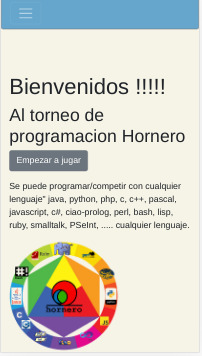
\includegraphics[width=6cm]{img/responsive.png}
\caption{Menu principal desplegado de un celular}
\label{1fig}
\end{center}
\end{figure}

%\begin{figure}
%\begin{center}
%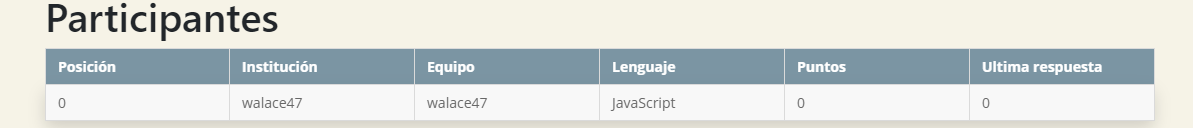
\includegraphics[width=8cm]{img/participantes-web.png}
%\caption{Tabla participantes vista web}
%\label{figWeb}
%\end{center}
%\end{figure}



Como se muestra en la Figura \ref{1fig} la nueva versión adapta en contenido a las dimensiones del dispositivo que se está utilizando, permitiendo que la visualización se acomode satisfactoriamente a un celular, tablet, monitor o proyector. Para lograr esto se usan librerías de css ({primefaces} \cite{bailey2015primefaces},
{boostrap 4} \cite{spurlock2013bootstrap}) que permiten diseñar alternativas para el despliegue de datos en diferentes pantallas. %Podemos ver la figura \ref{figWeb} que muestra una tabla como se despliega mediante una pantalla web mientras que la figura \ref{figMovil} se puede ver como se desplegaría esa misma tabla en un móvil.

%\begin{figure}
%\begin{center}
%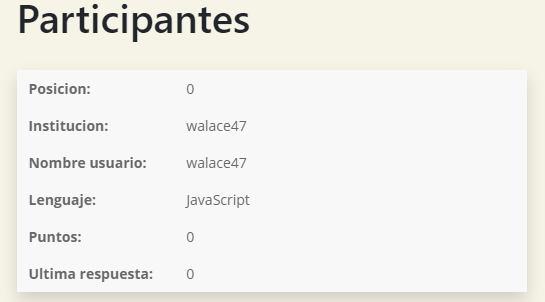
\includegraphics[width=8cm]{img/participantes-movil.png}
%\caption{Tabla participantes vista móvil}
%\label{figMovil}
%\end{center}
%\end{figure}
%agregar algo más

\begin{figure}
\begin{center}
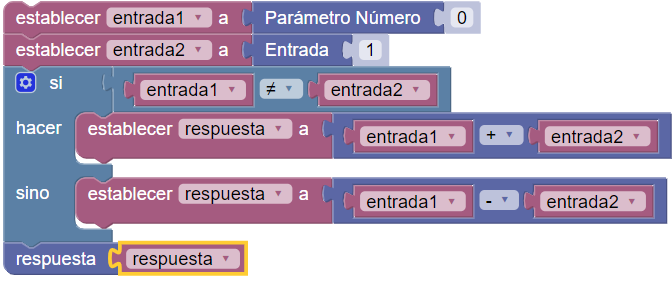
\includegraphics[width=8.5cm]{img/programa.png}
\end{center}
\caption{Programación Colaborativa basa en Bloques en Hornero}
\label{2fig}
\end{figure}



\subsection{Programación en Bloques}
%utilización de Blockly + referencia

Las tecnologías imponen nuevas realidades en la sociedad actual que requieren cambios dinámicos e innovadores, para poder mejorar los sistemas educativos \cite{weintrop2019block}.

%\begin{figure}
%\begin{center}
%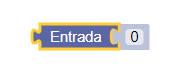
\includegraphics[width=5cm]{img/Entrada.png}
%\end{center}
%\caption{Entrada}
%\label{figEntrada}
%\end{figure}


La programación en la actualidad es un tema de mucha importancia que es básicamente uno de los pilares de nuestros avances tecnológicos actuales. Por ejemplo cada vez los componentes electrónicos son más genéricos y hay mucha necesidad de tener gente con capacidad de programarlos. Para incentivar el aprendizaje a la programación aparecen herramientas como la programación en bloques que facilita el acceso a chicos que cursan el primer o segundo nivel educativo.

%\begin{figure}
%\begin{center}
%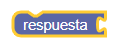
\includegraphics[width=4cm]{img/respuesta blockly.png}
%\end{center}
%\caption{Respuesta}
%\label{figRespuesta}
%\end{figure}
En hornero se implemento la librería \href{https://developers.google.com/blockly}{blockly} de google.
% Hace falta pononer como referencia a Blockly??????????
Sobre la cual se agregaron 3 nuevos bloques que permiten conectar con la competencia hornero o ejecución de manera local.
% Creo que sería mas ilustrativo una imagen en donde se resuelva un ejercicio simple y se utilicen los dos bloques
%\begin{enumerate}
%  \item Bloque retornar, este bloque tiene una conexión a la derecha ver figura \ref{figRespuesta} básicamente el valor que se inserte a lada derecha es el valor que a a enviar como respuesta del problema en caso de ser usado de manera local, se usa ese bloque para desplegar alguna respuesta.
  
%  \item Bloque entrada ver figura \ref{figEntrada} este bloque toma la entrada que envía el torneo en caso de probar el modo competencia, y en caso de estar en modo local te pide una entrada por teclado
%  \item Bloque parámetro entero ver figura \ref{figEntradaNumero} es equivalente al ítem anterior solo que espera un tipo entero.
%\end{enumerate}

%\begin{figure}
%\begin{center}
%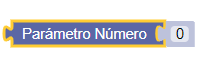
\includegraphics[width=5cm]{img/Entrada numero.png}
%\end{center}
%\caption{Entrada Numero}
%\label{figEntradaNumero}
%\end{figure}
    
\subsubsection{Ejecuciones}
El aplicativo tiene dos modos de ejecución, uno es el modo local lo que permite mediante interfaz de usuario probar entradas para tu algoritmo y retornara por pantalla la respuesta. Luego tiene el modo competitivo que permite jugar directamente contra hornero para competir con otros jugadores.
    
    
\subsubsection{Compilación bloques a texto}


La librería implementada, permite por defecto generar código en los siguiente lenguajes Javascript, Python, Dart, Lua, PHP y xml. Además se brinda una interfaz para generar código en otros lenguajes y producir código en bloques a través del lenguaje xml.


\subsection{Programación colaborativa}
Hornero, además, permite compartir un espacio de trabajo en grupos de 2 a 5 estudiantes. Todos los integrantes del equipo pueden cooperar, agregando, borrando o modificando bloques, en la construcción de cada solución.
Para lograr esto se implementan web-sockets en el servidor%con cada sala de programación de cada alumno
 usando la librería socket.io \cite{cadenhead2015socket}.


%Comparte el espacio/escritorio de Programación entre 2 a 5 estudiantes
% como es la dinámica y la experiencia de programar de forma Colaborativa


% -Descripción general de la herramienta
% 6/6 tiene esta sección

% Descripción general
% 2 o 3 párrafos



% Cierre de sección: Párrafo de forma
% 1 párrafo

\section{Requerimientos}
% Requerimientos necesarios para el uso de la herramienta/demo
% 2/6 tiene esta sección
Internet proyector, energía, celulares, tablets,

\section{Conclusiones}
Los conceptos de programación son incorporados de manera natural. La dinámica de los torneos partiendo de resolver cada problema varias veces, en papel para luego pasar al ambiente de programación en bloques, incita a los estudiantes a reutilizar el planteo resuelto en papel y transformarlo en bloques.  Asimismo, la posibilidad de trabajar de forma colaborativa permite a cada equipo llegar a soluciones construidas con el aporte de todos los integrantes.
%Trabajo futuro poder medir el aporte e suele medir cantidad y calidad
De esta manera se busca que los estudiantes aprendan a programar a través de la competencia y en un entorno distendido, introduciéndolos en una trama de aprendizaje compartida y de trabajo colaborativo. 


% Requerimientos necesarios para el uso de la herramienta/demo
% 1/6 tiene esta sección
 
\bibliographystyle{abbrv}
% 2/6 tiene esta sección
% 5 o 6 referencias

\bibliography{references}

\end{document}
% consulta de base de datos
% consultas dado un ejercicio que problema estuvo
% copiado de torneo